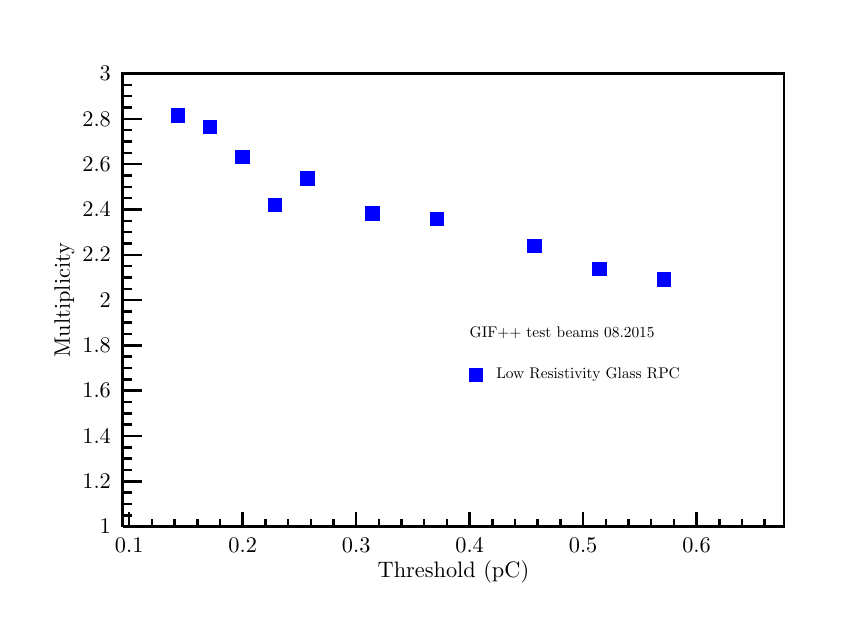
\begin{tikzpicture}
\pgfdeclareplotmark{cross} {
\pgfpathmoveto{\pgfpoint{-0.3\pgfplotmarksize}{\pgfplotmarksize}}
\pgfpathlineto{\pgfpoint{+0.3\pgfplotmarksize}{\pgfplotmarksize}}
\pgfpathlineto{\pgfpoint{+0.3\pgfplotmarksize}{0.3\pgfplotmarksize}}
\pgfpathlineto{\pgfpoint{+1\pgfplotmarksize}{0.3\pgfplotmarksize}}
\pgfpathlineto{\pgfpoint{+1\pgfplotmarksize}{-0.3\pgfplotmarksize}}
\pgfpathlineto{\pgfpoint{+0.3\pgfplotmarksize}{-0.3\pgfplotmarksize}}
\pgfpathlineto{\pgfpoint{+0.3\pgfplotmarksize}{-1.\pgfplotmarksize}}
\pgfpathlineto{\pgfpoint{-0.3\pgfplotmarksize}{-1.\pgfplotmarksize}}
\pgfpathlineto{\pgfpoint{-0.3\pgfplotmarksize}{-0.3\pgfplotmarksize}}
\pgfpathlineto{\pgfpoint{-1.\pgfplotmarksize}{-0.3\pgfplotmarksize}}
\pgfpathlineto{\pgfpoint{-1.\pgfplotmarksize}{0.3\pgfplotmarksize}}
\pgfpathlineto{\pgfpoint{-0.3\pgfplotmarksize}{0.3\pgfplotmarksize}}
\pgfpathclose
\pgfusepathqstroke
}
\pgfdeclareplotmark{cross*} {
\pgfpathmoveto{\pgfpoint{-0.3\pgfplotmarksize}{\pgfplotmarksize}}
\pgfpathlineto{\pgfpoint{+0.3\pgfplotmarksize}{\pgfplotmarksize}}
\pgfpathlineto{\pgfpoint{+0.3\pgfplotmarksize}{0.3\pgfplotmarksize}}
\pgfpathlineto{\pgfpoint{+1\pgfplotmarksize}{0.3\pgfplotmarksize}}
\pgfpathlineto{\pgfpoint{+1\pgfplotmarksize}{-0.3\pgfplotmarksize}}
\pgfpathlineto{\pgfpoint{+0.3\pgfplotmarksize}{-0.3\pgfplotmarksize}}
\pgfpathlineto{\pgfpoint{+0.3\pgfplotmarksize}{-1.\pgfplotmarksize}}
\pgfpathlineto{\pgfpoint{-0.3\pgfplotmarksize}{-1.\pgfplotmarksize}}
\pgfpathlineto{\pgfpoint{-0.3\pgfplotmarksize}{-0.3\pgfplotmarksize}}
\pgfpathlineto{\pgfpoint{-1.\pgfplotmarksize}{-0.3\pgfplotmarksize}}
\pgfpathlineto{\pgfpoint{-1.\pgfplotmarksize}{0.3\pgfplotmarksize}}
\pgfpathlineto{\pgfpoint{-0.3\pgfplotmarksize}{0.3\pgfplotmarksize}}
\pgfpathclose
\pgfusepathqfillstroke
}
\pgfdeclareplotmark{newstar} {
\pgfpathmoveto{\pgfqpoint{0pt}{\pgfplotmarksize}}
\pgfpathlineto{\pgfqpointpolar{44}{0.5\pgfplotmarksize}}
\pgfpathlineto{\pgfqpointpolar{18}{\pgfplotmarksize}}
\pgfpathlineto{\pgfqpointpolar{-20}{0.5\pgfplotmarksize}}
\pgfpathlineto{\pgfqpointpolar{-54}{\pgfplotmarksize}}
\pgfpathlineto{\pgfqpointpolar{-90}{0.5\pgfplotmarksize}}
\pgfpathlineto{\pgfqpointpolar{234}{\pgfplotmarksize}}
\pgfpathlineto{\pgfqpointpolar{198}{0.5\pgfplotmarksize}}
\pgfpathlineto{\pgfqpointpolar{162}{\pgfplotmarksize}}
\pgfpathlineto{\pgfqpointpolar{134}{0.5\pgfplotmarksize}}
\pgfpathclose
\pgfusepathqstroke
}
\pgfdeclareplotmark{newstar*} {
\pgfpathmoveto{\pgfqpoint{0pt}{\pgfplotmarksize}}
\pgfpathlineto{\pgfqpointpolar{44}{0.5\pgfplotmarksize}}
\pgfpathlineto{\pgfqpointpolar{18}{\pgfplotmarksize}}
\pgfpathlineto{\pgfqpointpolar{-20}{0.5\pgfplotmarksize}}
\pgfpathlineto{\pgfqpointpolar{-54}{\pgfplotmarksize}}
\pgfpathlineto{\pgfqpointpolar{-90}{0.5\pgfplotmarksize}}
\pgfpathlineto{\pgfqpointpolar{234}{\pgfplotmarksize}}
\pgfpathlineto{\pgfqpointpolar{198}{0.5\pgfplotmarksize}}
\pgfpathlineto{\pgfqpointpolar{162}{\pgfplotmarksize}}
\pgfpathlineto{\pgfqpointpolar{134}{0.5\pgfplotmarksize}}
\pgfpathclose
\pgfusepathqfillstroke
}
\definecolor{c}{rgb}{1,1,1};
\draw [color=c, fill=c] (0,0) rectangle (10,7.19298);
\definecolor{c}{rgb}{0,0,0};
\draw [c,line width=0.9] (1.2,0.863158) -- (1.2,6.61754) -- (9.6,6.61754) -- (9.6,0.863158) -- (1.2,0.863158);
\draw [c,line width=0.9] (1.2,0.863158) -- (1.2,6.61754) -- (9.6,6.61754) -- (9.6,0.863158) -- (1.2,0.863158);
\draw [c,line width=0.9] (1.2,0.863158) -- (1.2,6.61754) -- (9.6,6.61754) -- (9.6,0.863158) -- (1.2,0.863158);
\draw [c,line width=0.9] (1.2,0.863158) -- (1.2,6.61754) -- (9.6,6.61754) -- (9.6,0.863158) -- (1.2,0.863158);
\draw [c,line width=0.9] (1.2,0.863158) -- (9.6,0.863158);
\draw [c,line width=0.9] (1.28235,1.04442) -- (1.28235,0.863158);
\draw [c,line width=0.9] (1.57059,0.953789) -- (1.57059,0.863158);
\draw [c,line width=0.9] (1.85882,0.953789) -- (1.85882,0.863158);
\draw [c,line width=0.9] (2.14706,0.953789) -- (2.14706,0.863158);
\draw [c,line width=0.9] (2.43529,0.953789) -- (2.43529,0.863158);
\draw [c,line width=0.9] (2.72353,1.04442) -- (2.72353,0.863158);
\draw [c,line width=0.9] (3.01176,0.953789) -- (3.01176,0.863158);
\draw [c,line width=0.9] (3.3,0.953789) -- (3.3,0.863158);
\draw [c,line width=0.9] (3.58824,0.953789) -- (3.58824,0.863158);
\draw [c,line width=0.9] (3.87647,0.953789) -- (3.87647,0.863158);
\draw [c,line width=0.9] (4.16471,1.04442) -- (4.16471,0.863158);
\draw [c,line width=0.9] (4.45294,0.953789) -- (4.45294,0.863158);
\draw [c,line width=0.9] (4.74118,0.953789) -- (4.74118,0.863158);
\draw [c,line width=0.9] (5.02941,0.953789) -- (5.02941,0.863158);
\draw [c,line width=0.9] (5.31765,0.953789) -- (5.31765,0.863158);
\draw [c,line width=0.9] (5.60588,1.04442) -- (5.60588,0.863158);
\draw [c,line width=0.9] (5.89412,0.953789) -- (5.89412,0.863158);
\draw [c,line width=0.9] (6.18235,0.953789) -- (6.18235,0.863158);
\draw [c,line width=0.9] (6.47059,0.953789) -- (6.47059,0.863158);
\draw [c,line width=0.9] (6.75882,0.953789) -- (6.75882,0.863158);
\draw [c,line width=0.9] (7.04706,1.04442) -- (7.04706,0.863158);
\draw [c,line width=0.9] (7.33529,0.953789) -- (7.33529,0.863158);
\draw [c,line width=0.9] (7.62353,0.953789) -- (7.62353,0.863158);
\draw [c,line width=0.9] (7.91176,0.953789) -- (7.91176,0.863158);
\draw [c,line width=0.9] (8.2,0.953789) -- (8.2,0.863158);
\draw [c,line width=0.9] (8.48823,1.04442) -- (8.48823,0.863158);
\draw [c,line width=0.9] (1.28235,1.04442) -- (1.28235,0.863158);
\draw [c,line width=0.9] (8.48823,1.04442) -- (8.48823,0.863158);
\draw [c,line width=0.9] (8.77647,0.953789) -- (8.77647,0.863158);
\draw [c,line width=0.9] (9.0647,0.953789) -- (9.0647,0.863158);
\draw [c,line width=0.9] (9.35294,0.953789) -- (9.35294,0.863158);
\draw [anchor=base] (1.28235,0.539474) node[scale=0.807119, color=c, rotate=0]{0.1};
\draw [anchor=base] (2.72353,0.539474) node[scale=0.807119, color=c, rotate=0]{0.2};
\draw [anchor=base] (4.16471,0.539474) node[scale=0.807119, color=c, rotate=0]{0.3};
\draw [anchor=base] (5.60588,0.539474) node[scale=0.807119, color=c, rotate=0]{0.4};
\draw [anchor=base] (7.04706,0.539474) node[scale=0.807119, color=c, rotate=0]{0.5};
\draw [anchor=base] (8.48823,0.539474) node[scale=0.807119, color=c, rotate=0]{0.6};
\draw (5.4,0.287719) node[scale=0.807119, color=c, rotate=0]{Threshold (pC)};
\draw [c,line width=0.9] (1.2,0.863158) -- (1.2,6.61754);
\draw [c,line width=0.9] (1.44,0.863158) -- (1.2,0.863158);
\draw [c,line width=0.9] (1.32,1.00702) -- (1.2,1.00702);
\draw [c,line width=0.9] (1.32,1.15088) -- (1.2,1.15088);
\draw [c,line width=0.9] (1.32,1.29474) -- (1.2,1.29474);
\draw [c,line width=0.9] (1.44,1.4386) -- (1.2,1.4386);
\draw [c,line width=0.9] (1.32,1.58246) -- (1.2,1.58246);
\draw [c,line width=0.9] (1.32,1.72632) -- (1.2,1.72632);
\draw [c,line width=0.9] (1.32,1.87018) -- (1.2,1.87018);
\draw [c,line width=0.9] (1.44,2.01404) -- (1.2,2.01404);
\draw [c,line width=0.9] (1.32,2.15789) -- (1.2,2.15789);
\draw [c,line width=0.9] (1.32,2.30175) -- (1.2,2.30175);
\draw [c,line width=0.9] (1.32,2.44561) -- (1.2,2.44561);
\draw [c,line width=0.9] (1.44,2.58947) -- (1.2,2.58947);
\draw [c,line width=0.9] (1.32,2.73333) -- (1.2,2.73333);
\draw [c,line width=0.9] (1.32,2.87719) -- (1.2,2.87719);
\draw [c,line width=0.9] (1.32,3.02105) -- (1.2,3.02105);
\draw [c,line width=0.9] (1.44,3.16491) -- (1.2,3.16491);
\draw [c,line width=0.9] (1.32,3.30877) -- (1.2,3.30877);
\draw [c,line width=0.9] (1.32,3.45263) -- (1.2,3.45263);
\draw [c,line width=0.9] (1.32,3.59649) -- (1.2,3.59649);
\draw [c,line width=0.9] (1.44,3.74035) -- (1.2,3.74035);
\draw [c,line width=0.9] (1.32,3.88421) -- (1.2,3.88421);
\draw [c,line width=0.9] (1.32,4.02807) -- (1.2,4.02807);
\draw [c,line width=0.9] (1.32,4.17193) -- (1.2,4.17193);
\draw [c,line width=0.9] (1.44,4.31579) -- (1.2,4.31579);
\draw [c,line width=0.9] (1.32,4.45965) -- (1.2,4.45965);
\draw [c,line width=0.9] (1.32,4.60351) -- (1.2,4.60351);
\draw [c,line width=0.9] (1.32,4.74737) -- (1.2,4.74737);
\draw [c,line width=0.9] (1.44,4.89123) -- (1.2,4.89123);
\draw [c,line width=0.9] (1.32,5.03509) -- (1.2,5.03509);
\draw [c,line width=0.9] (1.32,5.17895) -- (1.2,5.17895);
\draw [c,line width=0.9] (1.32,5.32281) -- (1.2,5.32281);
\draw [c,line width=0.9] (1.44,5.46667) -- (1.2,5.46667);
\draw [c,line width=0.9] (1.32,5.61053) -- (1.2,5.61053);
\draw [c,line width=0.9] (1.32,5.75439) -- (1.2,5.75439);
\draw [c,line width=0.9] (1.32,5.89825) -- (1.2,5.89825);
\draw [c,line width=0.9] (1.44,6.04211) -- (1.2,6.04211);
\draw [c,line width=0.9] (1.32,6.18597) -- (1.2,6.18597);
\draw [c,line width=0.9] (1.32,6.32982) -- (1.2,6.32982);
\draw [c,line width=0.9] (1.32,6.47368) -- (1.2,6.47368);
\draw [c,line width=0.9] (1.44,6.61754) -- (1.2,6.61754);
\draw [anchor= east] (1.15,0.863158) node[scale=0.807119, color=c, rotate=0]{1};
\draw [anchor= east] (1.15,1.4386) node[scale=0.807119, color=c, rotate=0]{1.2};
\draw [anchor= east] (1.15,2.01404) node[scale=0.807119, color=c, rotate=0]{1.4};
\draw [anchor= east] (1.15,2.58947) node[scale=0.807119, color=c, rotate=0]{1.6};
\draw [anchor= east] (1.15,3.16491) node[scale=0.807119, color=c, rotate=0]{1.8};
\draw [anchor= east] (1.15,3.74035) node[scale=0.807119, color=c, rotate=0]{2};
\draw [anchor= east] (1.15,4.31579) node[scale=0.807119, color=c, rotate=0]{2.2};
\draw [anchor= east] (1.15,4.89123) node[scale=0.807119, color=c, rotate=0]{2.4};
\draw [anchor= east] (1.15,5.46667) node[scale=0.807119, color=c, rotate=0]{2.6};
\draw [anchor= east] (1.15,6.04211) node[scale=0.807119, color=c, rotate=0]{2.8};
\draw [anchor= east] (1.15,6.61754) node[scale=0.807119, color=c, rotate=0]{3};
\draw (0.458145,3.74035) node[scale=0.807119, color=c, rotate=90]{Multiplicity};
\definecolor{c}{rgb}{0,0,1};
\foreach \P in {(1.9,6.08345), (2.31176,5.93997), (2.72353,5.55854), (3.13529,4.9446), (3.54706,5.28394), (4.37059,4.84019), (5.19412,4.77165), (6.42941,4.4242), (7.25294,4.13801), (8.07647,4.00428)}{\draw[mark options={color=c,fill=c},mark
 size=2.402402pt,mark=square*] plot coordinates {\P};}
\definecolor{c}{rgb}{1,1,1};
\draw [color=c, fill=c] (5.5,2.51754) rectangle (7,3.59649);
\definecolor{c}{rgb}{0,0,0};
\draw [anchor= west] (5.5375,3.32675) node[scale=0.556634, color=c, rotate=0]{GIF++ test beams 08.2015};
\draw [anchor= west] (5.875,2.78728) node[scale=0.556634, color=c, rotate=0]{Low Resistivity Glass RPC};
\definecolor{c}{rgb}{0,0,1};
\foreach \P in {(5.6875,2.78728)}{\draw[mark options={color=c,fill=c},mark size=2.402402pt,mark=square*] plot coordinates {\P};}
\definecolor{c}{rgb}{0,0,0};
\draw [c,line width=0.9] (1.2,0.863158) -- (9.6,0.863158);
\draw [c,line width=0.9] (1.28235,1.04442) -- (1.28235,0.863158);
\draw [c,line width=0.9] (1.57059,0.953789) -- (1.57059,0.863158);
\draw [c,line width=0.9] (1.85882,0.953789) -- (1.85882,0.863158);
\draw [c,line width=0.9] (2.14706,0.953789) -- (2.14706,0.863158);
\draw [c,line width=0.9] (2.43529,0.953789) -- (2.43529,0.863158);
\draw [c,line width=0.9] (2.72353,1.04442) -- (2.72353,0.863158);
\draw [c,line width=0.9] (3.01176,0.953789) -- (3.01176,0.863158);
\draw [c,line width=0.9] (3.3,0.953789) -- (3.3,0.863158);
\draw [c,line width=0.9] (3.58824,0.953789) -- (3.58824,0.863158);
\draw [c,line width=0.9] (3.87647,0.953789) -- (3.87647,0.863158);
\draw [c,line width=0.9] (4.16471,1.04442) -- (4.16471,0.863158);
\draw [c,line width=0.9] (4.45294,0.953789) -- (4.45294,0.863158);
\draw [c,line width=0.9] (4.74118,0.953789) -- (4.74118,0.863158);
\draw [c,line width=0.9] (5.02941,0.953789) -- (5.02941,0.863158);
\draw [c,line width=0.9] (5.31765,0.953789) -- (5.31765,0.863158);
\draw [c,line width=0.9] (5.60588,1.04442) -- (5.60588,0.863158);
\draw [c,line width=0.9] (5.89412,0.953789) -- (5.89412,0.863158);
\draw [c,line width=0.9] (6.18235,0.953789) -- (6.18235,0.863158);
\draw [c,line width=0.9] (6.47059,0.953789) -- (6.47059,0.863158);
\draw [c,line width=0.9] (6.75882,0.953789) -- (6.75882,0.863158);
\draw [c,line width=0.9] (7.04706,1.04442) -- (7.04706,0.863158);
\draw [c,line width=0.9] (7.33529,0.953789) -- (7.33529,0.863158);
\draw [c,line width=0.9] (7.62353,0.953789) -- (7.62353,0.863158);
\draw [c,line width=0.9] (7.91176,0.953789) -- (7.91176,0.863158);
\draw [c,line width=0.9] (8.2,0.953789) -- (8.2,0.863158);
\draw [c,line width=0.9] (8.48823,1.04442) -- (8.48823,0.863158);
\draw [c,line width=0.9] (1.28235,1.04442) -- (1.28235,0.863158);
\draw [c,line width=0.9] (8.48823,1.04442) -- (8.48823,0.863158);
\draw [c,line width=0.9] (8.77647,0.953789) -- (8.77647,0.863158);
\draw [c,line width=0.9] (9.0647,0.953789) -- (9.0647,0.863158);
\draw [c,line width=0.9] (9.35294,0.953789) -- (9.35294,0.863158);
\draw [c,line width=0.9] (1.2,0.863158) -- (1.2,6.61754);
\draw [c,line width=0.9] (1.44,0.863158) -- (1.2,0.863158);
\draw [c,line width=0.9] (1.32,1.00702) -- (1.2,1.00702);
\draw [c,line width=0.9] (1.32,1.15088) -- (1.2,1.15088);
\draw [c,line width=0.9] (1.32,1.29474) -- (1.2,1.29474);
\draw [c,line width=0.9] (1.44,1.4386) -- (1.2,1.4386);
\draw [c,line width=0.9] (1.32,1.58246) -- (1.2,1.58246);
\draw [c,line width=0.9] (1.32,1.72632) -- (1.2,1.72632);
\draw [c,line width=0.9] (1.32,1.87018) -- (1.2,1.87018);
\draw [c,line width=0.9] (1.44,2.01404) -- (1.2,2.01404);
\draw [c,line width=0.9] (1.32,2.15789) -- (1.2,2.15789);
\draw [c,line width=0.9] (1.32,2.30175) -- (1.2,2.30175);
\draw [c,line width=0.9] (1.32,2.44561) -- (1.2,2.44561);
\draw [c,line width=0.9] (1.44,2.58947) -- (1.2,2.58947);
\draw [c,line width=0.9] (1.32,2.73333) -- (1.2,2.73333);
\draw [c,line width=0.9] (1.32,2.87719) -- (1.2,2.87719);
\draw [c,line width=0.9] (1.32,3.02105) -- (1.2,3.02105);
\draw [c,line width=0.9] (1.44,3.16491) -- (1.2,3.16491);
\draw [c,line width=0.9] (1.32,3.30877) -- (1.2,3.30877);
\draw [c,line width=0.9] (1.32,3.45263) -- (1.2,3.45263);
\draw [c,line width=0.9] (1.32,3.59649) -- (1.2,3.59649);
\draw [c,line width=0.9] (1.44,3.74035) -- (1.2,3.74035);
\draw [c,line width=0.9] (1.32,3.88421) -- (1.2,3.88421);
\draw [c,line width=0.9] (1.32,4.02807) -- (1.2,4.02807);
\draw [c,line width=0.9] (1.32,4.17193) -- (1.2,4.17193);
\draw [c,line width=0.9] (1.44,4.31579) -- (1.2,4.31579);
\draw [c,line width=0.9] (1.32,4.45965) -- (1.2,4.45965);
\draw [c,line width=0.9] (1.32,4.60351) -- (1.2,4.60351);
\draw [c,line width=0.9] (1.32,4.74737) -- (1.2,4.74737);
\draw [c,line width=0.9] (1.44,4.89123) -- (1.2,4.89123);
\draw [c,line width=0.9] (1.32,5.03509) -- (1.2,5.03509);
\draw [c,line width=0.9] (1.32,5.17895) -- (1.2,5.17895);
\draw [c,line width=0.9] (1.32,5.32281) -- (1.2,5.32281);
\draw [c,line width=0.9] (1.44,5.46667) -- (1.2,5.46667);
\draw [c,line width=0.9] (1.32,5.61053) -- (1.2,5.61053);
\draw [c,line width=0.9] (1.32,5.75439) -- (1.2,5.75439);
\draw [c,line width=0.9] (1.32,5.89825) -- (1.2,5.89825);
\draw [c,line width=0.9] (1.44,6.04211) -- (1.2,6.04211);
\draw [c,line width=0.9] (1.32,6.18597) -- (1.2,6.18597);
\draw [c,line width=0.9] (1.32,6.32982) -- (1.2,6.32982);
\draw [c,line width=0.9] (1.32,6.47368) -- (1.2,6.47368);
\draw [c,line width=0.9] (1.44,6.61754) -- (1.2,6.61754);
\draw [c,line width=0.9] (1.2,0.863158) -- (1.2,6.61754) -- (9.6,6.61754) -- (9.6,0.863158) -- (1.2,0.863158);
\draw [c,line width=0.9] (1.2,0.863158) -- (1.2,6.61754) -- (9.6,6.61754) -- (9.6,0.863158) -- (1.2,0.863158);
\end{tikzpicture}
